\section{Concept}

MagicVR was developed in a cooperation between Jerome Pönisch and Michael Maier.
This paper will be focused on the 3D-Gesture-Recognition done by Michael Maier while Jerome Pönisch\rq{}s paper will be focused on the 3D Art and FractTime-Animation effects.
%This section shall introduce in the general concept of MagicVR and the effects and animation part.

\subsection{The idea behind MagicVR}

The main idea of MagicVR is introducing the 3D-Gesture-Recognition module in a playful environment using important features of a virtual environment.
A user/player should be animated to use 3D-Gestures as interesting interaction technique rather than pushing buttons.
The virtual environment should help to gain the user/player\rq{}s interest and make him feel comfortable while experiencing the mixed reality world.
As User-Feedback it was decided to focus on animations and movements within the scene.

\begin{figure}[!ht]
    \centering
    \includegraphics[width=0.47\textwidth]{pictures/scene-overview-1.jpg}
    \caption{The scene shows Stonehenge with a fireplace and four pedestals.
    On each pedestal is a stone with a symbol that represents an element (from right to left: Fire, thunder, water, wind).}
    \label{fig:scene-overview-1}
\end{figure}

\begin{figure}[!ht]
    \centering
    \includegraphics[width=0.47\textwidth]{pictures/scene-overview-2.jpg}
    \caption{The user has to draw the symbol with the wand to activate the kind of magic of the respective element.
    The photo shows the scene after various magic spells have been executed. }
    \label{fig:scene-overview-2}
\end{figure}


\subsection{Movement Representation}

A movement is represented by a trajectory.~\autoref{fig:trajectory-example} shows examples of 2D trajectory definitions.
The same can be done for 3D space.
I use 2D trajectories in the trajectory examples of this paper because they are easier to visually perceive and compare.

\begin{description}
    \item{\textbf{Trajectory}} is a curve defined by a finite sequence of points
    with linear interpolation between consecutive points.
\end{description}

\begin{figure}[!htbp]
    \centering
    \subfigure[Pattern trajectory]{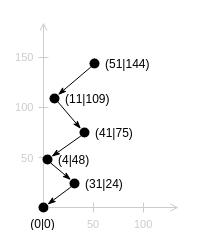
\includegraphics[width=0.23\textwidth]{pictures/lightning-trajectory.png}}
    \subfigure[Recorded trajectory]{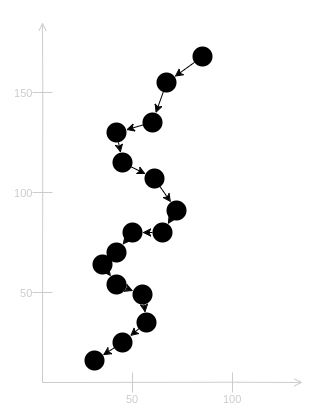
\includegraphics[width=0.23\textwidth]{pictures/possible-lightning-trajectory-input.png}}
    \caption{A pattern trajectory describes the ideal path of a movement.
    It is very unlikely that exactly the same trajectory is drawn and recorded.}
    \label{fig:trajectory-example}
\end{figure}


\subsection{Recording Movements}

In MagicVR the user plays a wizard that can do magic tricks by moving his magic
wand.
Therefore, the position of the wand is tracked over time to get a trajectory that represents the movement of the wand.
Those movements are used to interact with the scene of the application.
Only specific movements can trigger special events.
The scene (see~\autoref{fig:scene-overview-1}) contains four pedestals with a stone up on them.
On each stone is a different symbol.
If the user draws the symbol, an animaion is shown (see~\autoref{fig:scene-overview-2}).
To prevent the user from unintentionally triggering events by accidentally doing a specific movement, the user has to press the button on the backside of the wand.
The movement is only recorded while the button is pressed.
Thereby, only trajectories are recorded that are intended by the user.



\subsection{Definition Of Gestures}

A gesture describes a movement.
It is defined using a trajectory that describes the movement, preprocessing functions that transform trajectories and a comparison function that checks if two trajectories are similar.


\subsection{Detection Of Gestures}

Input trajectory (recorded movement) and pattern trajectory (description of a
specific movement) are preprocessed and compared by distance to each other.
Dependent on the result, a function is called to process the result (change the state of the application and trigger events (show effects)).~\autoref{fig:system-diagram} shows a diagram of this process.

\begin{figure}[!htbp]
    \centering
    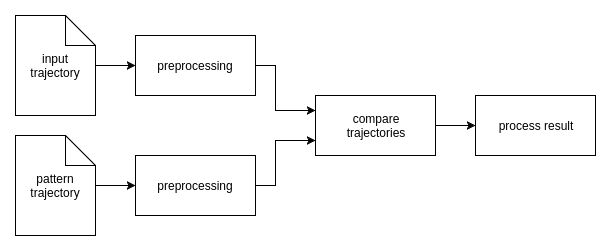
\includegraphics[width=0.5\textwidth]{pictures/system-diagram.png}
    \caption{System diagram}
    \label{fig:system-diagram}
\end{figure}


\subsection{Preprocessing}\label{subsec:preprocessing}

You can see in~\autoref{fig:trajectory-example} that most commonly input and pattern trajectory differ in the number of points, length/size, position, etc.
Distance functions may assume specific preconditions.
For example, some require that both trajectories have equal number of points or length.
The goal of the preprocessing (example shown in~\autoref{fig:preprocessing-steps}) is to prepare a trajectory for comparison with another trajectory (see~\autoref{fig:preprocessing-before-after}).
The appropriate preprocessing steps depend on the same factors as the limit that is used for~\nameref{subsubsec:deciding-similarity} including the preprocessing itself in that way that the preprocessing steps influence each other.
It is important in the process shown in~\autoref{fig:preprocessing-steps} to translate the trajectory to the origin before it is scaled.


\renewcommand\thesubfigure{\roman{subfigure}}

\begin{figure}[!htbp]
    \centering
    \subfigure[Calculate Minimum Bounding Sphere]{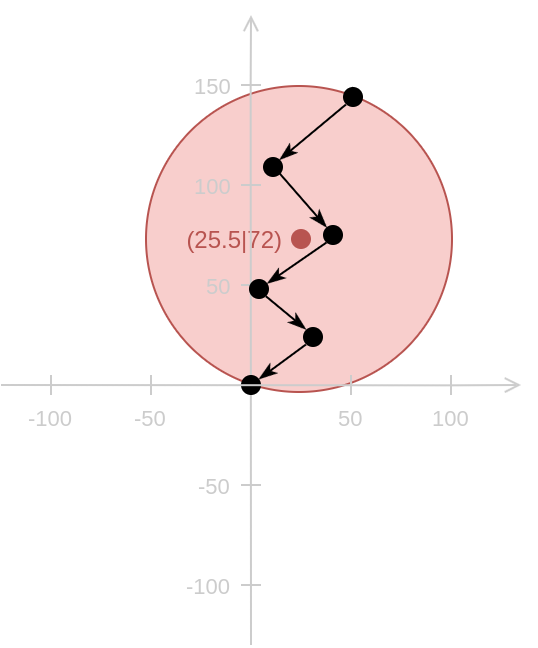
\includegraphics[width=0.156\textwidth]{pictures/min-bounding-sphere-preprocessing-1.png}\label{sfig:calculate-minimum-bounding-sphere}}
    \subfigure[Translate]{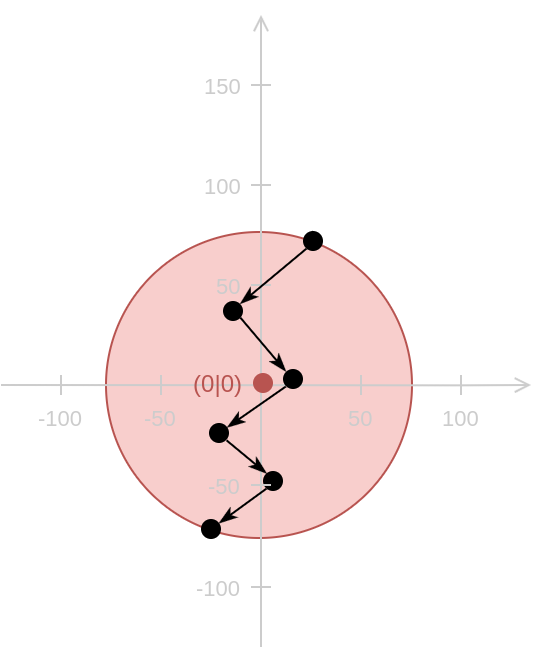
\includegraphics[width=0.156\textwidth]{pictures/min-bounding-sphere-preprocessing-2.png}\label{sfig:translate}}
    \subfigure[Scale]{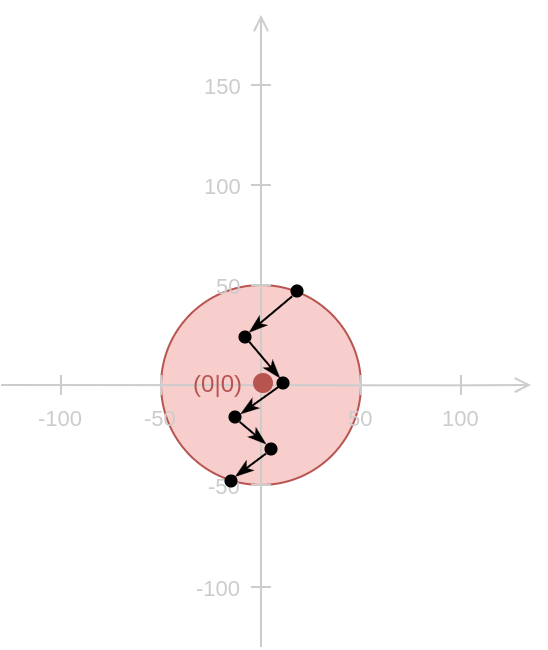
\includegraphics[width=0.156\textwidth]{pictures/min-bounding-sphere-preprocessing-3.png}\label{sfig:scale}}
    \caption{
    (\subref{sfig:calculate-minimum-bounding-sphere}) The smallest circle (hyper sphere) that contains all points of the trajectory is calculated.
    (\subref{sfig:translate}) Then the trajectory is moved so that the center of this circle is in the origin.
    (\subref{sfig:scale}) After that the trajectory is scaled so that the diameter of the circle is 100.
    }
    \label{fig:preprocessing-steps}
\end{figure}


\begin{figure}[!htbp]
    %    \centering
    \subfigure[Trajectories before preprocessing (pattern on the left, input on the right)]{
    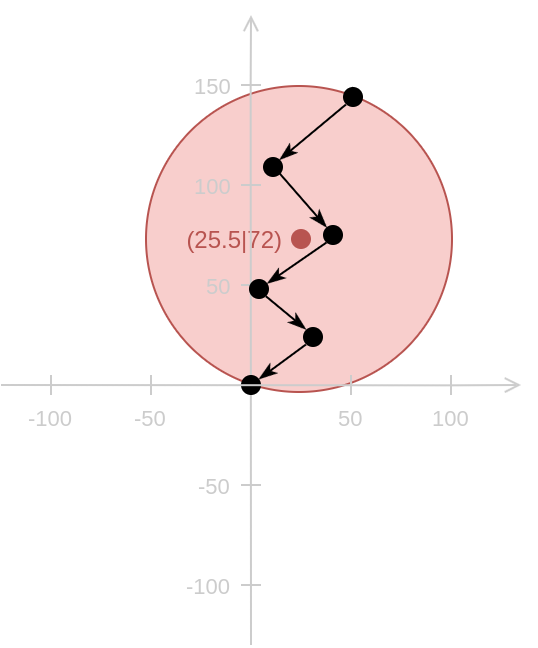
\includegraphics[width=0.26\textwidth]{pictures/min-bounding-sphere-preprocessing-1.png}
    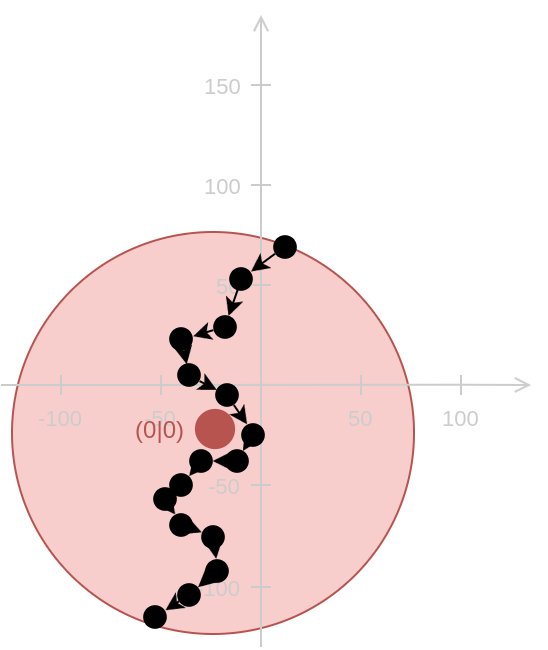
\includegraphics[width=0.26\textwidth]{pictures/preprocessing-input-1.png}
    \label{sfig:before-preprocessing}
    }
    \subfigure[Trajectories after preprocessing (pattern on the left, input on the right)]{
    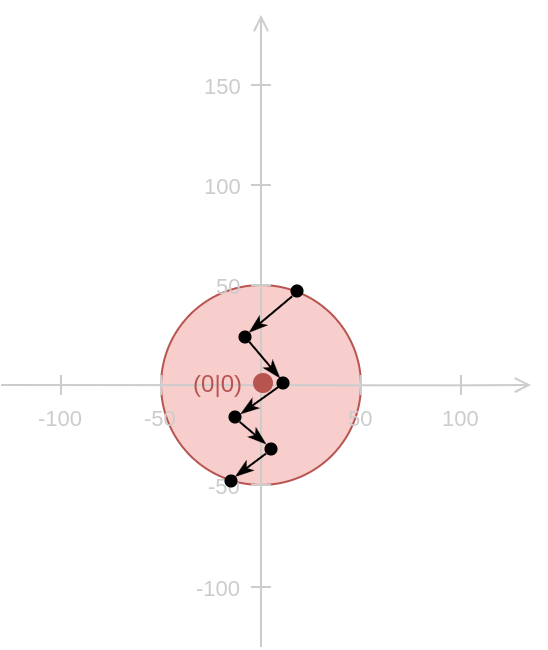
\includegraphics[width=0.26\textwidth]{pictures/min-bounding-sphere-preprocessing-3.png}
    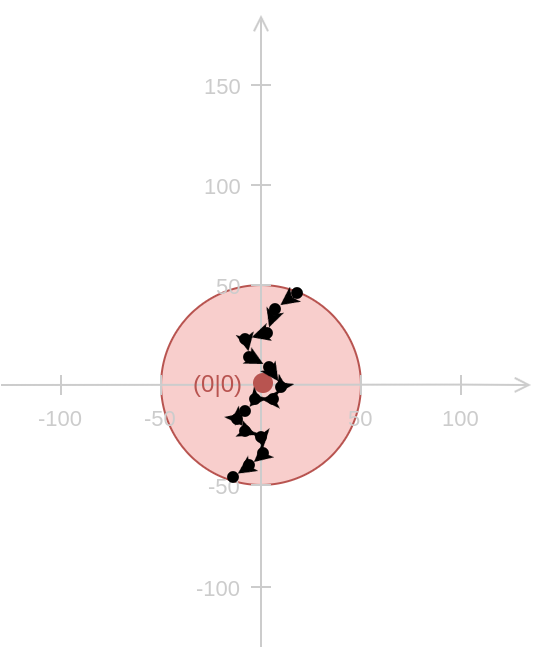
\includegraphics[width=0.26\textwidth]{pictures/preprocessing-input-3.png}
    \label{sfig:after-preprocessing}
    }
    \caption{
    (\subref{sfig:before-preprocessing}) The original trajectories differ in length/size and position.
    (\subref{sfig:after-preprocessing}) After the preprocessing they have similar length/size and the same position.
    }
    \label{fig:preprocessing-before-after}
\end{figure}


\subsection{Comparing Trajectories}\label{subsec:comparingTrajectories}
To check two trajectories for similarity we use a distance function to calculate the distance between them.
The distance is a scalar that indicates how similar two trajectories are.
We can decide similarity based on a limit.
If the distance is lower than the limit we consider two trajectories to be similar.

\subsubsection{Distance Function}
There is a wide range of distance functions to choose from.
Each has its pros and cons.
Good results are obtained using a \modifiedHausdorffDistFn (see~\autoref{fig:modified-hausdorff}).

\begin{figure}[!htbp]
    \centering
    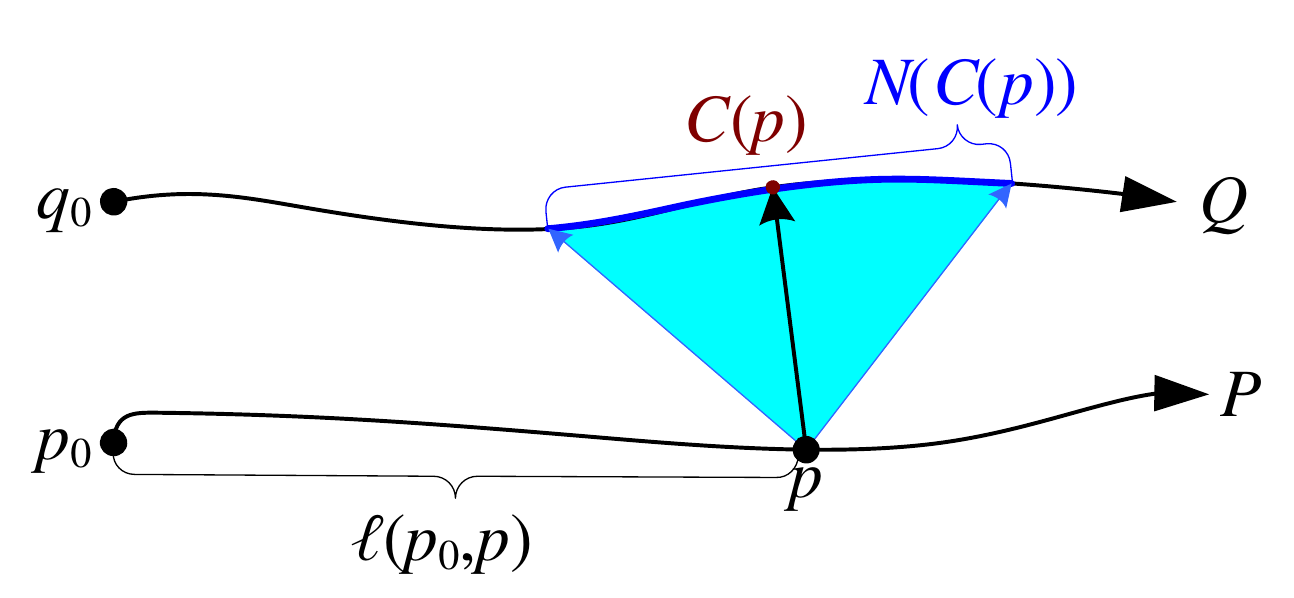
\includegraphics[width=0.5\textwidth]{pictures/modified-hausdorff-distance.png}
    \caption{
    The \modifiedHausdorffDistFn is a variant of the Hausdorff distance that takes the order of the points into account.
    It runs over all discrete points of both trajectories.
    The unmodified version of the Hausdorff distance determines the distance between each point and the other trajectory.
    The modified variant, on the other hand, only takes a subtrajectory - here \(N(C(p))\).
    For this purpose, the point \(C(p)\) on the other trajectory is determined for each point \(p\). \(C(p)\) is the point that lies at the same position relative to the length of the trajectory.
    \(N(C(p))\) defines the neighborhood of \(C(p)\). These are all points which are only a certain distance away from \(C(p)\) along the trajectory.
    The minimum distance to \(p\) is determined for this subtrajectory. I use the distance from point to distance, i. e. I consider the subtrajectory as a set of distances.
    So we now have a lot of space for each point of the discrete trajectory.
    The maximum of these distances is then the distance between the two trajectories.
    The order of the points is taken into account by \(C(p)\).
    }
    \label{fig:modified-hausdorff}
\end{figure}

\subsubsection{Deciding Similarity}\label{subsubsec:deciding-similarity}

We consider two trajectories to be similar if the distance is lower than the limit (see~\autoref{fig:deciding-similarity}).
Finding a good limit is crucial to avoid/reduce false positives and negatives.
If the limit is not tolerant enough, measuring inaccuracy of the input device recording the object position and natural small deviations during each movement execution will make it hard or impossible to recognize a movement.
If the limit is too tolerant we consider trajectories to be similar that should not.

Another important factor is the preprocessing of the trajectories.
Each preprocessing step might influence the distance (positive or negative).
The influence depends on the distance function.
Please also note that the distance might not grow linear.
For example, some distance functions use squared values.
Moreover, you should devote special attention to the scale of the trajectories, since the distance itself depends on it.\\

\noindent
Taken together, the limit depends on

\begin{itemize}
    %    \tightlist
    \item
    the measuring (in-) accuracy of the input device
    \item
    the minimum movement execution accuracy we claim from the user
    \item
    the preprocessing of the trajectories
    \item
    the scale of the trajectories
    \item
    the distance function
\end{itemize}


\begin{figure}[!htbp]
    \centering
    \subfigure[Similar trajectories]{
        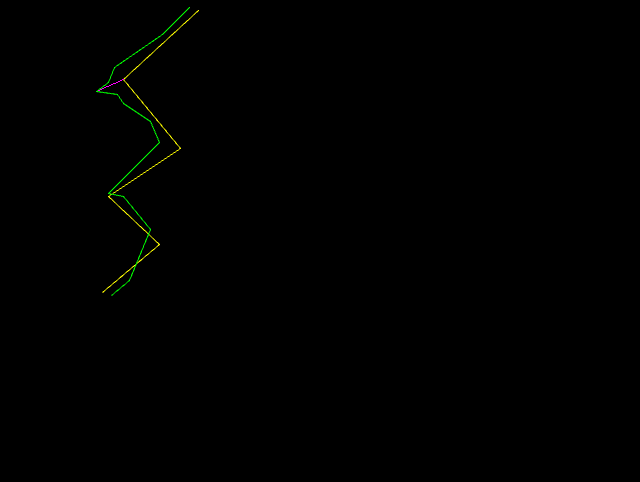
\includegraphics[width=0.5\textwidth]{pictures/similar-trajectories.png}
        \label{sfig:similar-trajectories}
    }
    \subfigure[Dissimilar trajectories]{
        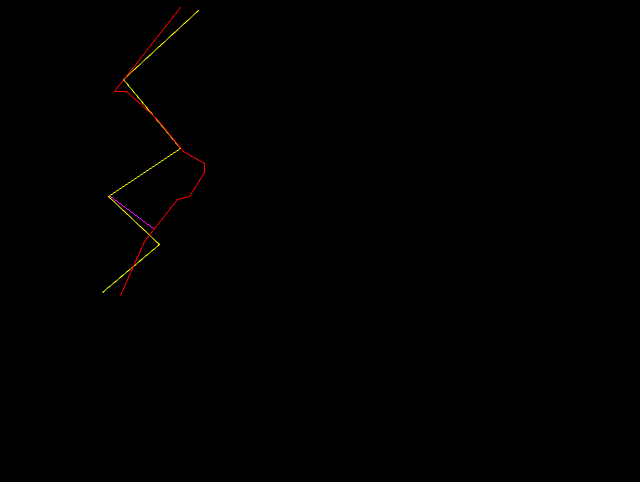
\includegraphics[width=0.5\textwidth]{pictures/dissimilar-trajectories.png}
        \label{sfig:dissimilar-trajectories}
    }
    \caption{
    Here you can see two screenshots of a 2D demo application of \trajecmp that visualizes the comparison of two standardized trajectories.
    The yellow trajectory represents the lightning pattern.
    (\subref{sfig:similar-trajectories})~shows a green trajectory, which has been classified as similar.
    In (\subref{sfig:dissimilar-trajectories}) you can see a red trajectory, which has been classified as dissimilar.
    The pink line represents the distance that has been calculated using the \modifiedHausdorffDistFn.
    }
    \label{fig:deciding-similarity}
\end{figure}
